\section{Designing Self-supervised Tasks}
\label{sec:designselftasks}

To alleviate human labor and avoid error propagation, self-supervised 
tasks emerged, which leverage dialogue-summary pairs without additional 
labels.  We divide such tasks into three sub-categories:
\begin{itemize}
	\item \textbf{Denoising tasks} are designed for eliminating noises 
in the input or penalizing negatives.
	\item \textbf{Masking and recovering tasks} mean that parts of the input are masked and the masked tokens are required to be predicted.
	\item \textbf{Dialogue tasks} refer to response selection and generation for better dialogue understanding.
\end{itemize}


\subsection{Denoising Tasks}

Denoising tasks focus on adding
noises to the dialogue input or output and aims at generating concise summaries by filtering out the noisy information, resulting in more robust dialogue 
summarization models.
\citet{zou2021unsupervised} used the original dialogue as output and trained a denoising auto-encoder which is capable of doing content compression for unsupervised dialogue summarization.
Noising operations, which include fragment insertion, utterance replacement, and
content retention, are applied together on each sample.
For a utterance $u_t$ in $D$, \textbf{fragment insertion} means that randomly sampled 
word spans from $u_t$ is inserted to $u_t$ for lengthening the original 
sequence.
\textbf{Utterance replacement} is that $u_t$ is replaced by another utterance $u_{t'}$ in $D$ and \textbf{content retention} means that $u_t$ is unchanged. 
\citet{chen2021simple} augmented dialogue data by swapping, deletion, insertion 
and substitution on utterance level and used the corresponding summary as 
the output, resulting in more various dialogue inputs for training the summarization model. 
\textbf{Swapping} and \textbf{deletion} aim to perturb discourse relations by randomly swapping two utterances in $D$ or deleting some utterances.
\textbf{Insertion} includes inserting repeated utterances that are chosen from $D$ randomly and inserting utterances with specific dialogue acts such as self-talk or hedge from a pre-extracted set, mimicking interruptions in natural dialogues.
\textbf{Substitution} replaces the chosen utterances in $D$ by utterances generated with a variant of text infilling task adopted in the BART pre-training process.
Only one operation is adopted to noise $D$ at a time, and these operations pay more attention to dialogue characteristics, such as the structure and context information.


This kind of task can be extended to learn beyond the denoising ability when 
combined with contrastive learning or classification tasks on positive and negative data. 
Contrastive learning trains the model to maximize 
the distance between positive data and negative data for learning more informative semantic representations, which extends the classification's ability on generation tasks.
\citet{liu2021topic} 
proposed {coherence detection} and {sub-summary generation} 
for implicitly modeling the topic change and handling information scattering 
problems. They cut the dialogue into snippets by sliding windows and 
separated the long summary into sentences as a first step.
\textbf{Coherence detection} is to train the encoder to distinguish 
a snippet with shuffled utterances from the original ordered one.
\textbf{Designated sub-summary generation} is to train the model to generate more related 
summaries by constructing negative samples with unpaired dialogue 
snippets and sub-summaries, where the positive pair is obtained 
by finding the snippet with the highest Rouge-2 recall for each sub-summary.
\citet{tang2021confit} also designated summaries where negative summaries are constructed for different error types, such as swapping the nouns for wrong reference and object errors, swapping verbs for circumstance errors and tense and modality errors, etc. Positive summaries are collected by back translation. The distance of decoder representations measures the contrastive loss.
They also considered the \textbf{token identification} task to identify whether two tokens belong to the same speaker based on their encoder representations.
\citet{zhao2021give} made improvements by \textbf{perturbing hidden representations} of 
the target summary for alleviating the exposure bias following~\citet{lee2020contrastive}, which is useful for conditional generation tasks.

\subsection{Masking and Recovering Tasks} 

Masking and recovering tasks 
are commonly used in pre-training for better language modeling by recovering the original dialogue and 
bear some resemblance to the noising operations. The main difference is that these tasks try to recover the original text given the corrupted one.
It can be divided into 
work-level and sentence-level by the granularity of masked contents.
Word-level masks for \textbf{pronouns}~\cite{khalifa2021bag}, \textbf{entities}~\cite{liu2022entity,khalifa2021bag}, 
\textbf{high-content tokens}~\cite{khalifa2021bag}, 
\textbf{roles}~\cite{qi2021improving} and \textbf{speakers}~\cite{zhong2021dialoglm} are 
considered in previous work, for a better understanding of the complicated speaker 
characteristics and capturing salient information. Words masked 
in \citet{khalifa2021bag}'s work was determined by POS tagger, 
named entity recognition or simple TF-IDF features. Although the lexical 
features and statistical features have been captured by pre-trained models 
for different words as mentioned in \secref{sec:feature}, predicting 
the specific content words under these features reversely given the dialogue context is still challenging and helpful to dialogue context modeling especially with models pre-trained on general text.
Utterance-level masking objective inspired by \textbf{Gap Sentence Prediction}~\cite{zhang2020pegasus} is adopted by~\citet{qi2021improving}. Key sentence selection from dialogues is done by a graph-based sorting algorithm TextRank and Maximum Margin Relevance. 
\citet{zhong2021dialoglm} introduced three new utterance-level tasks: 
\textbf{Turn splitting} is cutting a long utterance into multiple turns and 
adding ``[MASK]'' in front of each turn except the first one with 
the speaker. \textbf{Turn merging} is randomly merging consecutive turns 
into one turn and neglecting the speakers except the first one. 
And \textbf{turn permutation} means that utterances are randomly shuffled.

\subsection{Dialogue Tasks} 

There are also papers incorporating
well-known {dialogue tasks} into dialogue summarization. General \textbf{response 
selection} and \textbf{generation} models can be trained with unlabelled dialogues by 
simply regarding a selected utterance $u_t$ as the output and 
the utterances before it $u_{<t}$ as the input. Negative candidates for 
the selection task are the utterances randomly sampled from the whole corpus.
\citet{fuzw20} assumed that a superior summary is a representative of the 
original dialogue. So, either inputting $D$ or $Y$ is expected to achieve 
similar results on other tasks. In this way, the next utterance generation 
and classification tasks are acted like evaluators, to give guidance on better summary generation.
\citet{feigenblat-etal-2021-tweetsumm-dialog} trained response selection models for identifying salient utterances.
The intuition is that the removal of a salient utterance in dialogue context 
will lead to a dramatic drop in response selection, 
and these salient sentences are the same for summarization. 
Therefore, they regard the drop in probability as a saliency score to 
rank utterances and adopt the top 4 utterances as the
extractive summary, which can be further used to enhance abstractive 
results by appending it at the end of the input dialogue.

\subsection{Summary and Opinions}

\begin{figure}
	\centering
	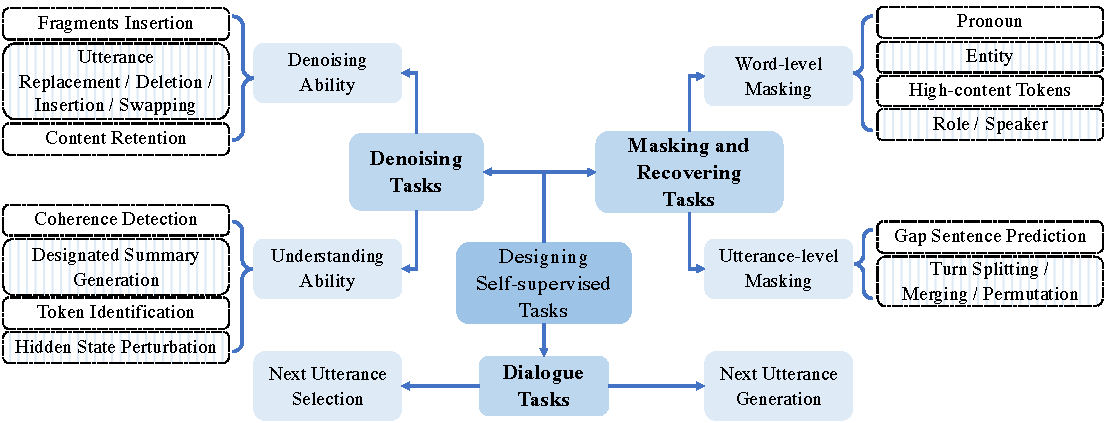
\includegraphics[scale=0.65]{fig/approach-tasks.pdf}
	\caption{A summary of self-supervised tasks.}
	\label{fig:app-task}
\end{figure}

The self-supervised tasks are summarized in Fig.~\ref{fig:app-task}. Most of them are adopted in two ways:
\begin{itemize}
	\item \textbf{Cooperating with the vanilla generation task under 
different training paradigms.}	
{Multi-task learning refers that the losses from self-supervised tasks are weighed summed with the vanilla generation for updating}~\cite{zhao2021give,fuzw20}, or updated sequentially in a batch~\cite{liu2021topic}. 
Pre-training with auxiliary tasks and then fine-tuning on dialogue summarization is also widely accepted~\cite{khalifa2021bag,qi2021improving}. 
The former is usually selected when the auxiliary training tasks are close to the summarization target. 
The latter one is chosen for learning more general representations, and is more flexible to use additional data in \secref{sec:useadddata}. 
	\item \textbf{Training an isolated model for different purposes.} 
The model is used as the summarization model directly~\cite{zou2021unsupervised, feigenblat-etal-2021-tweetsumm-dialog}, or as a trained labeler providing information for dialogue summarization~\cite{feigenblat-etal-2021-tweetsumm-dialog} with less artificial facts compared with \citet{feng2021language}. 
	
	

\end{itemize}


The advantages and disadvantages of designing self-supervised tasks are as follows:
\begin{itemize}
	\item[\Checkmark] Most self-supervised tasks take advantage of 
self-supervision to train the model. They don't need to go through
the expensive and time-consuming annotation process for collecting 
high-quality labels, and avoid the domain transfer problems 
of transferring labelers trained on the labeled domain to the target 
summarization domain.
	\item[\Checkmark] Useful representations are learned with these tasks by the summarization model directly or as an initial state for the summarization model, avoiding the error propagation caused by wrong labels. Although labeling tools such as POS tagger and TextRank are adopted, these predicted labels are not used as the training target or explicitly injected into the summarization model. They are just incorporated to find more effective self-supervisions.
	\item[\Checkmark] It's a good way to make full use of dialogue-summary 
pairs without additional labels, or even utilize pure dialogues without 
summaries.
	\item[\XSolidBrush] Although designing 
self-supervised tasks reduces the data pre-processing complexity, 
it increases the training time and computing costs with additional training targets 
on corresponding variations of the data.
	\item[\XSolidBrush] Different self-supervised tasks are not always 
compatible and controllable. It is challenging to design suitable tasks and 
find the best combination of tasks in different scenarios.
\end{itemize}


